\scanpage{262}
Démonstration calquée sur celle qui \unsure{sert|sort} dans le cas algébrique, \unsure{utilisant} RR analytique ....

\uline{Remarque} 1.10. Bien entendu, sous les conditions 1.8 \inserted{(ou de 1.9.)} on ne peut en général conclure que $f$ est projectif (globalement). Il en est cependant ainsi dans le cas suivant :

\figure{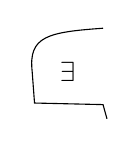
\begin{tikzpicture}[x=1cm,y=1cm]\node at(.45,.4){$\exists$};\draw (.9,.95)..controls(.2,.9)and(-.05,.85)..(0,.4)--(.03,0)--(.9,-.02)--(.95,-.2);\end{tikzpicture}}
partie discrète $T$ de $Y$ telle que

a) $X|(Y-T)\longrightarrow Y-T$ est \deleted{\uline{fini}} un isom

b) les anneaux locaux $\mathcal O_y$ $(y\in T)$ sont factoriels.

En effet, dans ce cas il est facile de construire un sous-\deleted{\unsure{ensemble}}\inserted{espace} analytique fermé $Z$ de $Y$, \uline{de support $\subset$} $T$, tel que $X$ soit $Y$-isom. à l'espace analytique \unsure{``déduit de $Y$'' en ``faisant éclater'' $Z$''}.

\uline{Remarque} 1.11. Sur les \unsure{variantes} analytique-formelle et algébrique formelle du th. envisagé. Il y a pour cette dernière une démonstration purement algébrique, utilisant \uline{Pic}, \deleted{\unsure{et}}\inserted{et} th. de finitude de Néron.

\mspage{261}
